\documentclass[]{book}
\usepackage{lmodern}
\usepackage{amssymb,amsmath}
\usepackage{ifxetex,ifluatex}
\usepackage{fixltx2e} % provides \textsubscript
\ifnum 0\ifxetex 1\fi\ifluatex 1\fi=0 % if pdftex
  \usepackage[T1]{fontenc}
  \usepackage[utf8]{inputenc}
\else % if luatex or xelatex
  \ifxetex
    \usepackage{mathspec}
  \else
    \usepackage{fontspec}
  \fi
  \defaultfontfeatures{Ligatures=TeX,Scale=MatchLowercase}
\fi
% use upquote if available, for straight quotes in verbatim environments
\IfFileExists{upquote.sty}{\usepackage{upquote}}{}
% use microtype if available
\IfFileExists{microtype.sty}{%
\usepackage{microtype}
\UseMicrotypeSet[protrusion]{basicmath} % disable protrusion for tt fonts
}{}
\usepackage{hyperref}
\hypersetup{unicode=true,
            pdftitle={Mesocosm User Manual},
            pdfauthor={Dr.~Nyssa Silbiger  and Danielle Barnas},
            pdfborder={0 0 0},
            breaklinks=true}
\urlstyle{same}  % don't use monospace font for urls
\usepackage{natbib}
\bibliographystyle{apalike}
\usepackage{longtable,booktabs}
\usepackage{graphicx}
% grffile has become a legacy package: https://ctan.org/pkg/grffile
\IfFileExists{grffile.sty}{%
\usepackage{grffile}
}{}
\makeatletter
\def\maxwidth{\ifdim\Gin@nat@width>\linewidth\linewidth\else\Gin@nat@width\fi}
\def\maxheight{\ifdim\Gin@nat@height>\textheight\textheight\else\Gin@nat@height\fi}
\makeatother
% Scale images if necessary, so that they will not overflow the page
% margins by default, and it is still possible to overwrite the defaults
% using explicit options in \includegraphics[width, height, ...]{}
\setkeys{Gin}{width=\maxwidth,height=\maxheight,keepaspectratio}
\IfFileExists{parskip.sty}{%
\usepackage{parskip}
}{% else
\setlength{\parindent}{0pt}
\setlength{\parskip}{6pt plus 2pt minus 1pt}
}
\setlength{\emergencystretch}{3em}  % prevent overfull lines
\providecommand{\tightlist}{%
  \setlength{\itemsep}{0pt}\setlength{\parskip}{0pt}}
\setcounter{secnumdepth}{5}
% Redefines (sub)paragraphs to behave more like sections
\ifx\paragraph\undefined\else
\let\oldparagraph\paragraph
\renewcommand{\paragraph}[1]{\oldparagraph{#1}\mbox{}}
\fi
\ifx\subparagraph\undefined\else
\let\oldsubparagraph\subparagraph
\renewcommand{\subparagraph}[1]{\oldsubparagraph{#1}\mbox{}}
\fi

%%% Use protect on footnotes to avoid problems with footnotes in titles
\let\rmarkdownfootnote\footnote%
\def\footnote{\protect\rmarkdownfootnote}

%%% Change title format to be more compact
\usepackage{titling}

% Create subtitle command for use in maketitle
\providecommand{\subtitle}[1]{
  \posttitle{
    \begin{center}\large#1\end{center}
    }
}

\setlength{\droptitle}{-2em}

  \title{Mesocosm User Manual}
    \pretitle{\vspace{\droptitle}\centering\huge}
  \posttitle{\par}
    \author{Dr.~Nyssa Silbiger and Danielle Barnas}
    \preauthor{\centering\large\emph}
  \postauthor{\par}
      \predate{\centering\large\emph}
  \postdate{\par}
    \date{2020-01-16}

\usepackage{booktabs}

\begin{document}
\maketitle

{
\setcounter{tocdepth}{1}
\tableofcontents
}
\chapter{Summary}\label{summary}

This manual describes the design, operation, and maintenance of the
mesocosm aquaria, located in the loading bay between Citrus Hall and
Eucalyptus Hall at California State University, Northridge, funded and
operated by Dr.~Nyssa Silbiger.

\chapter{Contacts}\label{contacts}

\begin{longtable}[]{@{}llll@{}}
\toprule
\begin{minipage}[b]{0.18\columnwidth}\raggedright\strut
Name\strut
\end{minipage} & \begin{minipage}[b]{0.25\columnwidth}\raggedright\strut
Involvement\strut
\end{minipage} & \begin{minipage}[b]{0.28\columnwidth}\raggedright\strut
Contact Information\strut
\end{minipage} & \begin{minipage}[b]{0.18\columnwidth}\raggedright\strut
Notes\strut
\end{minipage}\tabularnewline
\midrule
\endhead
\begin{minipage}[t]{0.18\columnwidth}\raggedright\strut
Nyssa Silbiger\strut
\end{minipage} & \begin{minipage}[t]{0.25\columnwidth}\raggedright\strut
System Design Asst. Professor, CSUN\strut
\end{minipage} & \begin{minipage}[t]{0.28\columnwidth}\raggedright\strut
\href{mailto:nyssa.silbiger@csun.edu}{\nolinkurl{nyssa.silbiger@csun.edu}}
818-677-4427\strut
\end{minipage} & \begin{minipage}[t]{0.18\columnwidth}\raggedright\strut
\strut
\end{minipage}\tabularnewline
\begin{minipage}[t]{0.18\columnwidth}\raggedright\strut
Danielle Barnas\strut
\end{minipage} & \begin{minipage}[t]{0.25\columnwidth}\raggedright\strut
System Installation and Maintenance Silbiger Lab Tech, CSUN\strut
\end{minipage} & \begin{minipage}[t]{0.28\columnwidth}\raggedright\strut
\href{mailto:danielle.barnas@csun.edu}{\nolinkurl{danielle.barnas@csun.edu}}\strut
\end{minipage} & \begin{minipage}[t]{0.18\columnwidth}\raggedright\strut
\strut
\end{minipage}\tabularnewline
\begin{minipage}[t]{0.18\columnwidth}\raggedright\strut
Louis Dang\strut
\end{minipage} & \begin{minipage}[t]{0.25\columnwidth}\raggedright\strut
Systems Engineer\strut
\end{minipage} & \begin{minipage}[t]{0.28\columnwidth}\raggedright\strut
\href{mailto:louis@aqualogicinc.com}{\nolinkurl{louis@aqualogicinc.com}}\strut
\end{minipage} & \begin{minipage}[t]{0.18\columnwidth}\raggedright\strut
\href{http://www.aqualogicinc.com}{www.aqualogicinc.com}\strut
\end{minipage}\tabularnewline
\begin{minipage}[t]{0.18\columnwidth}\raggedright\strut
Bill Krohmer\strut
\end{minipage} & \begin{minipage}[t]{0.25\columnwidth}\raggedright\strut
Administrative Operations\strut
\end{minipage} & \begin{minipage}[t]{0.28\columnwidth}\raggedright\strut
\href{mailto:william.krohmer@csun.edu}{\nolinkurl{william.krohmer@csun.edu}}\strut
\end{minipage} & \begin{minipage}[t]{0.18\columnwidth}\raggedright\strut
\strut
\end{minipage}\tabularnewline
\begin{minipage}[t]{0.18\columnwidth}\raggedright\strut
Science Shop\strut
\end{minipage} & \begin{minipage}[t]{0.25\columnwidth}\raggedright\strut
CSUN College of Science and Math Machine Shop\strut
\end{minipage} & \begin{minipage}[t]{0.28\columnwidth}\raggedright\strut
818-677-3055\strut
\end{minipage} & \begin{minipage}[t]{0.18\columnwidth}\raggedright\strut
Location: EH 2014 Available M-Th 0600-1630
\href{http://www.csun.edu/science-mathematics/science-shop}{www.csun.edu/Science-Shop}\strut
\end{minipage}\tabularnewline
\begin{minipage}[t]{0.18\columnwidth}\raggedright\strut
Perry Martin\strut
\end{minipage} & \begin{minipage}[t]{0.25\columnwidth}\raggedright\strut
Supervising Plumber, PPM\strut
\end{minipage} & \begin{minipage}[t]{0.28\columnwidth}\raggedright\strut
\href{mailto:perry.martin@csun.edu}{\nolinkurl{perry.martin@csun.edu}}
818-677-2222 (PPM) 818-677-2237\strut
\end{minipage} & \begin{minipage}[t]{0.18\columnwidth}\raggedright\strut
\strut
\end{minipage}\tabularnewline
\begin{minipage}[t]{0.18\columnwidth}\raggedright\strut
Will Moran\strut
\end{minipage} & \begin{minipage}[t]{0.25\columnwidth}\raggedright\strut
Network Engineer, CSUN IT\strut
\end{minipage} & \begin{minipage}[t]{0.28\columnwidth}\raggedright\strut
\href{mailto:will.moran@csun.edu}{\nolinkurl{will.moran@csun.edu}}
818-677-6273\strut
\end{minipage} & \begin{minipage}[t]{0.18\columnwidth}\raggedright\strut
\strut
\end{minipage}\tabularnewline
\begin{minipage}[t]{0.18\columnwidth}\raggedright\strut
Willy Martinez\strut
\end{minipage} & \begin{minipage}[t]{0.25\columnwidth}\raggedright\strut
Lead Electrician, PPM Electric Shop\strut
\end{minipage} & \begin{minipage}[t]{0.28\columnwidth}\raggedright\strut
\href{mailto:willy.martinez@csun.edu}{\nolinkurl{willy.martinez@csun.edu}}
818-677-6273\strut
\end{minipage} & \begin{minipage}[t]{0.18\columnwidth}\raggedright\strut
\strut
\end{minipage}\tabularnewline
\begin{minipage}[t]{0.18\columnwidth}\raggedright\strut
Neptune Systems\strut
\end{minipage} & \begin{minipage}[t]{0.25\columnwidth}\raggedright\strut
Apex Support Team\strut
\end{minipage} & \begin{minipage}[t]{0.28\columnwidth}\raggedright\strut
\href{mailto:support@neptunesystems.com}{\nolinkurl{support@neptunesystems.com}}\strut
\end{minipage} & \begin{minipage}[t]{0.18\columnwidth}\raggedright\strut
\href{http://www.neptunesystems.com}{www.neptunesystems.com}\strut
\end{minipage}\tabularnewline
\begin{minipage}[t]{0.18\columnwidth}\raggedright\strut
Dickson Lab\strut
\end{minipage} & \begin{minipage}[t]{0.25\columnwidth}\raggedright\strut
Seawater CO2 CRMs\strut
\end{minipage} & \begin{minipage}[t]{0.28\columnwidth}\raggedright\strut
\href{mailto:co2crms@ucsd.edu}{\nolinkurl{co2crms@ucsd.edu}}
858-534-2582\strut
\end{minipage} & \begin{minipage}[t]{0.18\columnwidth}\raggedright\strut
Marine Physical Lab, Scripps Institution of Oceanography University of
CA, San Diego 9500 Gilman Drive, La Jolla, CA 92093-0244 USA\strut
\end{minipage}\tabularnewline
\bottomrule
\end{longtable}

\hypertarget{system-details}{\chapter{System
Details}\label{system-details}}

\textbf{Contents}\\
- \protect\hyperlink{Aquaria_System_List}{\textbf{Aquaria System}}\\
-
\protect\hyperlink{Filtration_and_Recirculation_System}{\textbf{Filtration
and Recirculation System}}\\
- \protect\hyperlink{System_Operation_Parameters}{\textbf{System
Operational Parameters}}\\
- \protect\hyperlink{Apex_Connection_Series}{\textbf{Apex Connection
Series}}\\
- \protect\hyperlink{EB832_Outlet_Connections}{\textbf{EB832 Outlet
Connections}} - \protect\hyperlink{Water_Flow_Operation}{\textbf{Water
Flow Operation}}

 \textbf{Aquaria System Component List}

\begin{itemize}
\tightlist
\item
  Experimental Tanks (21.25'' x 12.5'' x 13.5''H) - Per tank:\\
\item
  1 Submersible powerhead pump
  (\href{https://github.com/SilbigerLab/Mesocosm_User_Manual/blob/master/Manuals/Hydor_Nano_Pump.pdf}{Hydor
  Nano Koralia 240 powerhead})\\
\item
  1 200 W Heater
  (\href{https://github.com/SilbigerLab/Mesocosm_User_Manual/blob/master/Manuals/Hydor_Heater.pdf}{Hydor
  aquarium heater})\\
\item
  1 Light
  (\href{https://github.com/SilbigerLab/Mesocosm_User_Manual/blob/master/Manuals/Apex_Halo.pdf}{Halo
  Basic M-110})\\
\item
  1 Temperature probe (Apex)\\
\item
  1 pH probe (Apex)\\
\item
  1 Solenoid valve for pH (Apex)\\
\item
  3 Flow sensors (Apex, FS-25 1/4" fitting, flow rates from 3-12 GPH
  (12-45 LPH))\\
\item
  1 Main Supply line: ``N''\\
\item
  1 Solenoid Supply line: ``S''\\
\item
  1 Drain line: ``D''\\
\item
  1 Gate valve (solenoid for water inflow)\\
\item
  1 VDM
  (\href{https://github.com/SilbigerLab/Mesocosm_User_Manual/blob/master/Manuals/VDM_manual.pdf}{Apex
  Variable Dimming Module}, 1 unit for 4 tanks)\\
\item
  1 FMM (\href{https://www.neptunesystems.com/getstarted/fmk/}{Apex
  Fluid Metering Module})\\
\item
  1 PM1
  (\href{https://github.com/SilbigerLab/Mesocosm_User_Manual/blob/master/Manuals/PM1_manual.pdf}{Apex
  Probe Module 1})\\
\item
  1 Base Unit
  (\href{https://github.com/SilbigerLab/Mesocosm_User_Manual/blob/master/Manuals/Apex_Comprehensive_Reference_Manual.pdf}{Apex}
  processing unit, 1 unit for 4 tanks)\\
\item
  1 EB832
  (\href{https://github.com/SilbigerLab/Mesocosm_User_Manual/blob/master/Manuals/EB832_Guide.pdf}{Apex
  8-outlet EnergyBar}, 1 unit for 2 tanks)\\
\item
  1 CO2 regulator valve
  (\href{https://github.com/SilbigerLab/Mesocosm_User_Manual/blob/master/Manuals/Tunze_CO2_Regulator.pdf}{Tunze
  pH Controller Set, pressure reducing valve 7077/3})\\
\item
  1 Industrial Grade Carbon Dioxide,
  \href{https://www.airgas.com/product/Gases/Industrial-Application-Gases/Carbon-Dioxide---Industrial/p/CD\%2050}{50
  pound cylinder}
\end{itemize}

 \textbf{Filtration and Recirculation}
\href{https://github.com/SilbigerLab/Mesocosm_User_Manual/blob/master/Manuals/Filtration_Skid_Build_Package.pdf}{\textbf{System}}
\textbf{Component List}

\begin{itemize}
\tightlist
\item
  Sump (66.25'' x 31.5'' x 21''H)\\
\item
  Chiller
  (\href{https://github.com/SilbigerLab/Mesocosm_User_Manual/blob/master/Manuals/AquaLogic_Chiller.pdf}{AquaLogic
  Multi-Temp and Titan Series})\\
\item
  Heat Pump
  (\href{https://github.com/SilbigerLab/Mesocosm_User_Manual/blob/master/Manuals/AquaLogic_Chiller.pdf}{AquaLogic
  Multi-Temp and Titan Series})\\
\item
  PM1
  (\href{https://github.com/SilbigerLab/Mesocosm_User_Manual/blob/master/Manuals/PM1_manual.pdf}{Apex
  Probe Module 1})\\
\item
  Water pump
  (\href{https://github.com/SilbigerLab/Mesocosm_User_Manual/blob/master/Manuals/Complete_Cascade.pdf}{PerformancePro
  Cascade pump})\\
\item
  UV Sterilizer (Comet Series 95 Watt Lamp)\\
\item
  PhosBan chemical filter
  (\href{https://github.com/SilbigerLab/Mesocosm_User_Manual/blob/master/Manuals/Phosban_Reactor.pdf}{PhosBan
  Reactor 550})\\
\item
  Air compressor\\
\item
  Airstones (4 units on 4 outflow tubes)\\
\item
  Carbon filter cells (3 units, CF28AC,28in, ActC)\\
\item
  Mesh filter (8 units, Matala Filter Media, interchanged 4 Blue high
  density and 4 Black low density sheets)
\end{itemize}

 \textbf{System Operational Parameters}

\begin{itemize}
\tightlist
\item
  This is a closed loop system where water from each individual tank
  will recirculate back to a main holding reservoir (sump).\\
\item
  Normal High Tide operating water level is approximately 12.5``H for a
  total water volume of 14.37 gal per tank (287.4 gal total for the
  20-tank-system).\\
\item
  Normal Low Tide operating water level is approximately 4``H for a
  total water volume of 4.60 gal per tank (92.0 gal total for the
  20-tank-system).\\
\item
  Excess water volume to sump at low tide is 9.77 gal per tank (195.4
  gal total for the 20-tank-system).\\
\item
  Normal sump operating water level is 7" water in the filter cell
  compartment, which has an approximate volume of 82.32 gal. Sump
  freeboard volume is 107.39 gal.\\
\item
  Aquaria drain line is in line with a 30 gal sump pump, which will draw
  water from the aquaria drain line and pump water to the sump.\\
\item
  Sump is in line with a secondary holding tank for sump overflow at Low
  Tide.

  \begin{itemize}
  \tightlist
  \item
    195.4 gal returning to sump in a Low Tide scenario
  \item
    30 gal in sump pump
  \item
    107.39 gal in sump (freeboard volume)
  \item
    58.01 gal necessarily pumped to secondary holding tank\\
  \end{itemize}
\item
  Flow rate for each tank is 2-6 GPH (See
  \href{chapters/06-tidal_manipulation.md}{Tidal Manipulation} for
  specific flow rates).\\
\item
  Chiller is plumbed inline with the
  \href{https://github.com/SilbigerLab/Mesocosm_User_Manual/blob/master/Manuals/Filtration_Skid_Build_Package.pdf}{filtration
  skid} which includes mechanical/biological filtration as well as UV
  sterilization (chemical filtration).\\
\item
  One main pump recirculates the water flow throughout the experimental
  tanks and the main holding reservoir.\\
\item
  Each tank has an immersion heater that allows tank temperatures to be
  set 15 degF (8.3 degC) above the main holding tank reservoir.

  \begin{itemize}
  \tightlist
  \item
    \textbf{Note: The tank needs to have low flow or be static in order
    to heat up to a desired temp. Once the temperature has been reached
    then it can be set to normal operating flow through mode.}\\
  \end{itemize}
\item
  A small sumbersible powerhead in each tank provides water circulation
  throughout the tank.\\
\item
  Each tank has (2) supply lines, each with (1) Neptune Systems flow
  sensor and (1) needle valve for incoming flow rate control, and (1)
  gate solenoid valve in line with (1) supply line for tidal effect.
  Each tank also has (2) drain lines with (1) flow sensor in line with
  (1) needle valve for outgoing flow rate control. Incoming and outgoing
  flow rates have to be manually adjusted for the tidal effect.\\
\item
  Flow metered water lines

  \begin{itemize}
  \tightlist
  \item
    N: Main supply
  \item
    S: Solenoid-controlled supply
  \item
    D: Drain\\
  \end{itemize}
\item
  Tidal effect

  \begin{itemize}
  \tightlist
  \item
    outgoing tide: incoming flow rate (N + S) is lower than outgoing
    flow rate (D).
  \item
    incoming tide: incoming flow rate (N + S) is greater than outgoing
    flow rate (D).
  \item
    Note: The tank will not be completely empty during low tide events
    to prevent the recirculating powerhead from running dry.\\
  \end{itemize}
\item
  Each tank has (1) CO2 supply line with an airstone connected to (1)
  Neptune Systems solenoid valve to control and lower pH in tanks.\\
\item
  CO2 scrubber comprised of an air compressor connected to a Phosban
  Reactor will bubble air into the sump to bring pH to ambient or
  near-ambient conditions in the holding reservoir.\\
\item
  Each tank has individual LED lighting, which can be controlled for
  white or blue light by specific times or natural daily light cycles.\\
\item
  Certain tank conditions can be controlled via Neptune Systems Apex
  Controllers. Each Apex controls (4) tanks.\\
\item
  Controllable parameters are pH, temperature, tidal effect, and
  lighting.
\end{itemize}

 \textbf{Apex Connection Series}

\begin{itemize}
\tightlist
\item
  Each EnergyBar connects to the Base Unit with an AquaBus cable via the
  AquaBus Ports for power. (2) EB832 units connect to (1) Base Unit.\\
\item
  Each CO2 Solenoid valve connects to the EnergyBar via the DC24
  Accessory Port on the side of the EB832. (2) Solenoid valves connect
  in (1) EB832.\\
\item
  (1)PM1 connects to (1) EnergyBar with an AquaBus cable via the AquaBus
  Ports, and all PM1 modules connect in series with each other for
  power.\\
\item
  VDM connects to the last PM1 in series with an AquaBus cable via the
  AquaBus Ports for power.\\
\item
  Temperature probes connect to the PM1 Temp Port or the Base Unit Temp
  Port. (1) Temperature probe in each PM1, and (1) Temperature probe in
  the Base Unit.\\
\item
  pH probes connect to the PM1 pH/ORP Port or the Base Unit pH/ORP Port.
  Push the BNC female connector of the probe on to the male connector
  and turn 1/4 turn clockwise to lock the connector in place. (1) pH
  probe in each PM1, and (1) pH probe in the Base Unit.\\
\item
  \href{https://github.com/SilbigerLab/Mesocosm_User_Manual/tree/394a3f7d9fed8765e4152f9fdd11d00a2ea87a93/Manuals/HALO_Quick_Start_Guide.pdf}{Halo
  light} connects to the VDM or Base Unit via the V1/V2 or V3/V4 Port.
  (2) Light connections in the VDM and (2) Light connections in the Base
  Unit.\\
\item
  (1)FMM connects to (1) EnergyBar (whichever EB832 is not powering the
  PM1 modules) with an AquaBus cable via the AquaBus Ports, and all FMM
  connect in series with each other for power.\\
\item
  (3)Flow sensors connect to each FMM via (3) of the numbered ports.
\end{itemize}

 \textbf{EB832 Outlet Connections}

Note: Each horizontal row on an EB832 corresponds to one tank, yielding
4 outlets per aquarium. Current outlet order, left to right:

\begin{enumerate}
\def\labelenumi{\arabic{enumi}.}
\tightlist
\item
  200W Heater
\item
  Hydor Powerhead
\item
  Water supply line ``S'' Solenoid
\item
  Halo Light
\end{enumerate}

 \textbf{Water Flow Operation}

\begin{itemize}
\tightlist
\item
  Inflow from the filtration sump to the mesocosm tanks

  \begin{itemize}
  \tightlist
  \item
    Water from the chiller can be directed either back into the sump
    (the bypass t-valve is parallel to the pvc, opening flow to the
    sump, and the tank t-valve is perpendicular to the pvc, closing flow
    to the tanks) or to the mesocosm tanks (the bypass valve is angled
    to allow partial flow to the sump and tanks, and the tank valve is
    parallel or angled with the pvc, opening flow to the tanks).
  \item
    The bypass valve is used to regulate the line pressure going back to
    the mesocosm tanks. The more closed, the higher the pressure in the
    line, and the more open, the lower the pressure.
  \item
    The chiller has a safety flow switch that requires a minimum flow
    rate for the chiller to operate, so the bypass valve can be used to
    regulate the chiller flow as well as the container flow.
  \end{itemize}
\item
  Outflow from the mesocosm tanks to the filtration sump

  \begin{itemize}
  \tightlist
  \item
    Water from the tanks drains to an outdoor underground sump pump,
    which will automatically pump water out when a certain water level
    is reached. This water can be directed either back into the sump
    (the sump inflow t-valve is opened parallel to the pvc, allowing
    flow to the three dump pipes into the filtration skid), or if you
    intend to drain water in the event of a water change or the end of
    an experiment, water can be directed to a drain port (the sump
    inflow valve is closed and the drain t-valve along the South wall is
    opened parallel to the pvc).
  \end{itemize}
\item
  Overflow from sump to secondary containment

  \begin{itemize}
  \tightlist
  \item
    When mesocosm water level falls from a high tide to low tide
    sequence, more water will drain to the sump than what the main sump
    can individually hold. Excess water can be redirected from the sump
    (S1) to the secondary containment (S2) by opening the S2 inflow
    t-valve (allows simultaneous flow of filtered, chilled water to both
    S2 and the mesocosm tanks), and the overflow t-valve (allows
    continuous flow exchange between S1 and S2).
  \end{itemize}
\end{itemize}

\chapter{Inventory}\label{inventory}

\textbf{Contents}\\
- \protect\hyperlink{Experimental_Mesocosm}{\textbf{Experimental
Mesocosm}} - \protect\hyperlink{Filtration}{\textbf{Filtration}} -
\protect\hyperlink{Spare_Items}{\textbf{Spare Items}}

 \textbf{Experimental Mesocosm}

\begin{longtable}[]{@{}lll@{}}
\toprule
Item & Quantity & Purchase Replacement\tabularnewline
\midrule
\endhead
Experimental Aquarium & 20 &\tabularnewline
Aquarium Lid & 20 &\tabularnewline
200W Heater & 20 &
\href{https://www.amazon.com/Hydor-Submersible-Glass-Aquarium-Heater/dp/B00061UQ7K}{\$24.99
Amazon}\tabularnewline
Suction Heater Slip & 40 &\tabularnewline
Halo Light & 20 &
\href{https://www.amazon.com/Aquatic-Life-Halo-Basic-Fixture/dp/B00T6FGDJW}{\$299.99
Amazon}\tabularnewline
Halo Light Power Cords & 20 &\tabularnewline
Hydor Powerhead & 20 &
\href{https://www.amazon.com/Hydor-Koralia-Nano-Aquarium-Circulation/dp/B0036S70ZG/ref=sr_1_2?keywords=hydor+powerhead\&qid=1572981966\&s=pet-supplies\&sr=1-2}{\$34.99
Amazon}\tabularnewline
Temperature Probe & 20 &
\href{https://www.bulkreefsupply.com/temperature-probe-neptune-systems.html}{\$29.95
Bulk Reef Supply}\tabularnewline
Suction Temperature Probe Slip & 20 &\tabularnewline
pH Probe & 20 &
\href{https://www.bulkreefsupply.com/lab-grade-double-junction-ph-probe-neptune-systems.html}{\$74.95
Bulk Reef Supply}\tabularnewline
Suction pH Probe Slip & 20 &\tabularnewline
Salinity Probe & 5 &
\href{https://www.bulkreefsupply.com/neptune-systems-lab-grade-conductivity-probe.html}{124.95
Bulk Reef Supply}\tabularnewline
pH and Salinity Calibration Pack \(7,10\) & 10 &
\href{https://www.bulkreefsupply.com/probe-calibration-kit-ph-7-0-ph-10-0-salinity-53000us-neptune-systems.html}{\$6.85
Bulk Reef Supply}\tabularnewline
CO2 Solenoid Valve & 20 &
\href{https://www.bulkreefsupply.com/sv-1-solenoid-valve-neptune-systems.html}{\$29.95
Bulk Reef Supply}\tabularnewline
FS-25 1/4" Flow Sensor & 60 &
\href{https://www.bulkreefsupply.com/1-4-flow-sensor-fs25-neptune-systems.html}{\$19.95
Bulk Reef Supply}\tabularnewline
Flow Solenoid/Gate Valve & 20 &
\href{https://www.electricsolenoidvalves.com/1-4-120v-ac-electric-plastic-solenoid-valve/}{\$16.99
Electric Solenoid Valves}\tabularnewline
Inflow Seawater Tubing & 40 &\tabularnewline
Inflow CO2 Tubing & 20 &\tabularnewline
Airstone & 20 &
\href{https://www.amazon.com/Pawfly-Cylinder-Diffuser-Airstones-Hydroponics/dp/B075QCWGZQ/ref=sr_1_5?crid=3EXLLKKDA2NYZ\&keywords=airstones+for+aquariums\&qid=1572983301\&sprefix=airstone\%2Caps\%2C197\&sr=8-5}{\$5.99x10pack
Amazon}\tabularnewline
Inflow Tubing Stand & 40 &\tabularnewline
VDM & 5 &
\href{https://www.bulkreefsupply.com/led-pumps-control-module-vdm-neptune-systems.html}{\$99.95
Bulk Reef Supply}\tabularnewline
FMM & 20 &
\href{https://www.bulkreefsupply.com/fmm-fluid-monitoring-module-neptune-systems.html}{\$99.95
Bulk Reef Supply}\tabularnewline
PM1 & 16 &
\href{https://www.bulkreefsupply.com/ph-orp-probe-module-pm1-neptune-systems.html}{\$84.95
Bulk Reef Supply}\tabularnewline
Display Module & 1 &
\href{https://www.bulkreefsupply.com/apex-display-module-neptune-systems.html}{\$99.95
Bulk Reef Supply}\tabularnewline
Apex Base Unit & 5 &
\href{https://www.bulkreefsupply.com/apex-controller-base-unit-neptune-systems.html}{\$399.95
Bulk Reef Supply}\tabularnewline
Apex EB832 & 10 &
\href{https://www.bulkreefsupply.com/energybar-832-neptune-systems.html}{\$249.95
Bulk Reef Supply}\tabularnewline
Tunze CO2 Regulator Valve & 1 &\tabularnewline
180gal Sump & 1 &\tabularnewline
Chiller & 1 &\tabularnewline
\bottomrule
\end{longtable}

 \textbf{Filtration}

\begin{longtable}[]{@{}lll@{}}
\toprule
Item & Quantity & Purchase Replacement\tabularnewline
\midrule
\endhead
PhosBan Reactor 550 & 1 &
\href{https://www.bulkreefsupply.com/phosban-reactor-550.html}{\$85.14
Bulk Reef Supply}\tabularnewline
PhosBan CDX Carbon Dioxide Absorption Media 3L & 1 &
\href{https://www.bulkreefsupply.com/cdx-carbon-dioxide-adsorption-media-two-little-fishies.html}{\$44.38
Bulk Reef Supply}\tabularnewline
Cascade Water Pump & 1 &\tabularnewline
UV Sterilizer & 1 &\tabularnewline
UV Light & 1 &\tabularnewline
Air Pump & 1 &\tabularnewline
Air Pump tubing to Phosban Reactor 3/8" ID x 10' & 2 &
\href{https://www.homedepot.com/p/UDP-3-8-in-I-D-x-1-2-in-O-D-x-10-ft-Clear-Vinyl-Tubing-T10006008/304185141}{\$4.93
Home Depot}\tabularnewline
Airflow Tubing 3/16" ID x 8' & 4 &
\href{https://www.petsmart.com/fish/filters-and-pumps/air-and-water-pumps/grreat-choice-airline-tubing-5202767.html}{\$2.69
Petsmart}\tabularnewline
Airstone & 4 &\tabularnewline
Carbon Filter Cell & 3 &\tabularnewline
Matala Filter, High Density (Blue) & 4 &\tabularnewline
Matala Filter, Low Density (Black) & 4 &\tabularnewline
\bottomrule
\end{longtable}

 \textbf{Spare Items}

\begin{longtable}[]{@{}ll@{}}
\toprule
Item & Quantity\tabularnewline
\midrule
\endhead
Solenoid Valve & 4\tabularnewline
Flow Solenoid/Gate Valve & 5\tabularnewline
Halo Light & 1\tabularnewline
Airstone & 29\tabularnewline
Halo Light-to-Light Cable & 16\tabularnewline
pH Calibration Pack \(7,10\) & 3\tabularnewline
Salinity Calibration Pack \(53,000 uS\) & 3\tabularnewline
FS-25 1/4" Flow Sensor & 0\tabularnewline
pH Probe & 0\tabularnewline
Conductivity Probe & 0\tabularnewline
Temperature Probe & 0\tabularnewline
Hydor Powerhead & 0\tabularnewline
\bottomrule
\end{longtable}

\chapter{Start-up Guide}\label{start-up-guide}

\textbf{Contents}\\
- \protect\hyperlink{Basic_Operation}{\textbf{Basic Operation}}\\
- \protect\hyperlink{Filtration}{\textbf{Filtration}}\\
- \protect\hyperlink{System}{\textbf{System}} -
\protect\hyperlink{Sump_Flow}{\textbf{Sump Flow}} -
\protect\hyperlink{CO2_Scrubber}{\textbf{CO2 Scrubber}}

 \textbf{Basic Operation}

\begin{enumerate}
\def\labelenumi{\arabic{enumi}.}
\tightlist
\item
  Operating water level in the filtration sump should be 7" in the
  filter cell compartment.
\item
  Overflow water from the tanks will feed down to the outside
  underground sump pump, then into to the filtration skid inside the
  Citrus Hall Field Room. The water will flow through mesh filters and
  be pumped through carbon filters, the UV sterilizer, and chiller, then
  back to the tanks.
\end{enumerate}

 \textbf{Filtration}

\begin{itemize}
\tightlist
\item
  Biological and Mechanical Filtration: Water from the Mesocosm tanks is
  pumped into the sump by passing through 6 mesh filters. These filters
  have an accumulated biofilm to biologically filter the water before it
  enters the sump.
\item
  Chemical and Mechanical Filtration: Water in the sump is pulled
  through the three carbon filters with mesh filter sleeves by a pump
  and pushed up into the UV sterilizer, where is is then directed
  through the chiller chamber.
\end{itemize}

 \textbf{System Details}

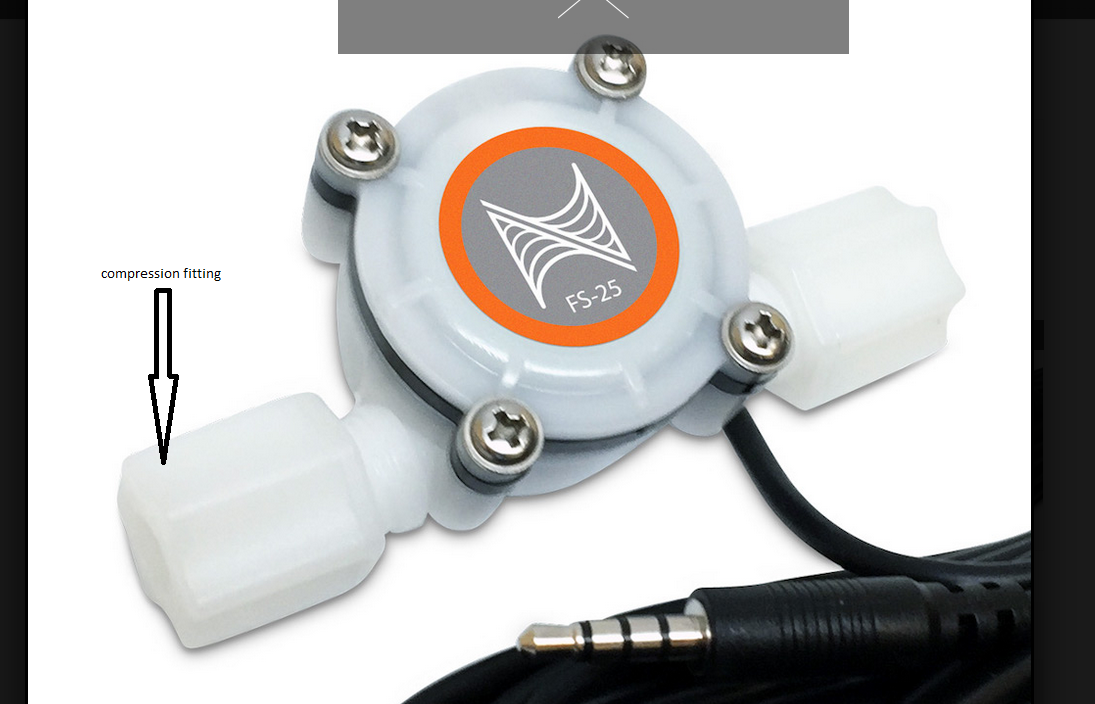
\includegraphics{images/flowmeter.PNG} a

 \textbf{Sump Flow}

\begin{enumerate}
\def\labelenumi{\arabic{enumi}.}
\tightlist
\item
  Filling the mesocosm tanks

  \begin{enumerate}
  \def\labelenumii{\arabic{enumii}.}
  \tightlist
  \item
    Make sure the drain valve located under each tank is closed (turned
    clockwise all the way, finger-tight).
  \item
    Open the N flow valve for each tanks (and S flow valve if you're
    turning the Solenoid ON to fill the tanks).
  \item
    To open flow from the sump to the tanks, first
  \item
    Fill each rack one at a time and make sure rack and filtration skid
    flows are balanced before moving on to the next rack.
  \item
    Make sure the complete system reaches equilibrium in standard
    recirculation mode before setting up the tidal cycle.
  \end{enumerate}
\item
  Set flow in tanks

  \begin{enumerate}
  \def\labelenumii{\arabic{enumii}.}
  \tightlist
  \item
    Calculate your desired residence time. When full, each tank holds 55
    liters, so divide 55L by your desired residence time and use that
    estimated value as your flow rate. Example: for a RT of 8 hours:
    55L/8hr = 6.88 L/hr or 114.67 mL/min
  \item
    If you have an acceptable range for your residence time, set flow
    rate to within that range, as close to your desired flow as
    possible. Example: for a RT of 7.5-8.5 hours: RT = 6.47-7.33 L/hr or
    107.83-122.17 mL/min
  \item
    Use the Neptune Systems flow meters as a guide for setting the flow,
    but for the most accurate flow rates, use a graduated cylinder to
    estimate flow into each tank.
  \item
    Flow will slightly change throughout the day, so it is recommended
    to set flow twice per day: once in the morning and once in the
    afternoon/evening.
  \end{enumerate}
\end{enumerate}

 \textbf{CO2 Scrubber} 1. Connect tubing to the back outtake port of the
white airpump and to the phosban reactor, leaving the intake port on the
airpump free 1.

\chapter{Tidal Manipulation}\label{tidal-manipulation}

Controling the tidal cycle of each experimental tank with the Apex. This
is achieved by manipulating the incoming and outgoing flow rates of each
individual tank with the needle valves described in the
\protect\hyperlink{system-details}{System Details}, and setting the
ON/OFF time cycle of the supply line with the solenoid. The basic
procedure is outlined below.

\begin{enumerate}
\def\labelenumi{\arabic{enumi}.}
\tightlist
\item
  Set the flow rate of the supply line N{[}\#{]}FLW (without the
  solenoid), for example 10.5 Liters/Hr, by slowly turning the black
  knob counterclockwise to increase flow or clockwise to decrease flow.

  \begin{enumerate}
  \def\labelenumii{\arabic{enumii}.}
  \tightlist
  \item
    You can view rates on the Fusion dashboard.
  \item
    Note that the Apex controller has some lag time in registering the
    flow rate after the valve has been adjusted, and the delay can be up
    to 30 seconds or more, so make small adjustments and monitor the
    change on Fusion.
  \item
    Once the rate is set you should check periodically to make sure the
    rate has not changed both on Fusion and by using a graduated
    cylinder and a timer.
  \end{enumerate}
\item
  Adjust the outgoing flow rate of the drain line D{[}\#{]}FLW higher
  than the N{[}\#{]}FLW, for example 15 Liters/Hr.

  \begin{enumerate}
  \def\labelenumii{\arabic{enumii}.}
  \tightlist
  \item
    With the above condition, the outgoing flow rate is higher than the
    incoming, so this will create a low tide effect over a 5-5.25 hr
    period.
  \end{enumerate}
\item
  To create a high tide effect, change the setting of SOL-TNK-\#
  (outlets 3 and 7 on each EB832) to ON on the Fusion dashboard, then
  manually turn on and adjust the flow rate of the supply line
  S{[}\#{]}FLW , for example 10 Liters/Hr.\\
\item
  Once the S{[}\#{]}FLW is set, change the setting of SOL-TNK-\# to AUTO
  on the Fusion dashboard.

  \begin{enumerate}
  \def\labelenumii{\arabic{enumii}.}
  \tightlist
  \item
    With the above condition, the total incoming flow rate (N+S) is
    higher thatn the outgoing (D), so this will create a high tide
    effect over a 5-5.25 hr period.
  \item
    For a constant ON/OFF cycle over a 12.5 hour period, the Advanced
    program should look like the program below:
  \end{enumerate}
\end{enumerate}

Fallback ON\\
Osc 000:00/375:00/375:00 then ON

\begin{enumerate}
\def\labelenumi{\arabic{enumi}.}
\tightlist
\item
  In the event the EnergyBar loses connection with the Apex Base,
  ``Fallback ON'' will keep the solenoid open, allowing water to
  continuously flow from S{[}\#{]}FLW.\\
\item
  The oscillate (Osc) command as written will open flow from
  S{[}\#{]}FLW for 6.25 hours, initiating the High Tide scenario, then
  close for 6.25 hours, initiating the Low Tide scenario. This will
  provide the effect of two high and two low tides of a semidiurnal
  tidal cycle over a 25 hour period.

  \begin{enumerate}
  \def\labelenumii{\arabic{enumii}.}
  \tightlist
  \item
    Using the flow rates stated above, each tidal shift will last 5.25
    hours and maintain the tide height for 1 hour.
  \end{enumerate}
\end{enumerate}

For more advanced programming features, see the
\href{https://github.com/SilbigerLab/Mesocosm_User_Manual/tree/7503b88686aef920c4a4ed473b1efe37b34dae10/Manuals/Apex_Comprehensive_Reference_Manual.pdf}{Comprehensive
Manual}. Start on Page 65 for Seasonal Features and Moon cycles.

\chapter{Controlling pH}\label{controlling-ph}

The pH is controlled with the addition of CO\textsubscript{2} gas to the
system. The gas is delivered to the tank by air stone and is controlled
through the Apex Controls with a solenoid valve connected to the EB832.

\begin{enumerate}
\def\labelenumi{\arabic{enumi}.}
\tightlist
\item
  Once the CO\textsubscript{2} regulator is connected to a tank, open
  the main tank valve.
\item
  Use the pressure adjusting screw (larger knob in front with Tunze
  label) to adjust the pressure (in bar) on the pressure gauge. Turning
  \textbf{clockwise to open}, thus increasing pressure, while turning
  \textbf{counterclockwise to close}, thus reducing pressure.
\item
  The pressure should be set to 0.5 up to 1 bar on the gauge
  (\textasciitilde{}7.5psi) - ideally 0.6 bar.
\item
  Open the fine adjustment valve (smaller valve next to the tubing
  connecting the regulator to the tanks) to allow gas to the tank
  solenoid. If the pressure on the gauge is too high this may prevent
  the CO\textsubscript{2} solenoid from completely closing, which will
  inject excess CO\textsubscript{2} into the system.
\item
  Programming the solenoid for a consistent pH: pH-TNK-\#
\end{enumerate}

Control type: pH Control\\
Probe name: pH\\
Fallback: OFF\\
High Value: 8.2\\
Low Value: 7.9\\
On when: High

\begin{enumerate}
\def\labelenumi{\arabic{enumi}.}
\setcounter{enumi}{5}
\tightlist
\item
  Programming the solenoid for diel variance:
\end{enumerate}

\begin{itemize}
\tightlist
\item
  Using Advanced programming and Virtual outlets
\item
  Create a unique virtual outlet for every time block which requires a
  different pH, and for every tank/probe which requires that pH
  treatment. *Virtual Outlet Example (for the 6 hours between 6:31am and
  12:30pm, the CO2 solenoid will dose CO2 into tank 1 while the probe
  reads 8.10 or above): Fallback OFF Set OFF If Time 06:31 to 12:30 Then
  ON If pH-1 \textless{} 8.10 Then OFF
\end{itemize}

*Advanced Program Example (Every 6 hours, the pH setpoint changes, and
each of the four time block has a unique virtual outlet name, as
presented below in the four programming lines. The CO2 solenoid will
dose the tank when the conditions of the virtual outlet program are
met): Fallback OFF Set OFF If Output pH\_1\_630 = ON Then ON If Output
pH\_1\_1230 = ON Then ON If Output pH\_1\_1830 = ON Then ON If Output
pH\_1\_0030 = ON Then ON

Refer to
\href{https://github.com/SilbigerLab/Mesocosm_User_Manual/tree/7503b88686aef920c4a4ed473b1efe37b34dae10/Manuals/Apex_Comprehensive_Reference_Manual.pdf}{Comprehensive
Manual} for set point programming.

\chapter{Apex Programming Guide}\label{apex-programming-guide}

Recommendations for programming the Apex aquarium controllers designated
for the Silbiger Lab Mesocosm, located in the loading bay between Citrus
Hall and Eucalyptus Hall at California State University, Northridge.
These recommendations are for maintaining tanks at ambient conditions.
Changes should be made according to your study aims.

The following are using the numbered system of Apex1\_39106, controlling
tanks 1-4. All methods are transferrable across all 5 Apex controllers
to yield the same outcome in all 20 tanks, or change programs for varied
results.

\textbf{Contents}\\
- \protect\hyperlink{Programm_Screen}{**Accessing the Programming Edit
Screen in Apex} - \protect\hyperlink{Probes}{\textbf{Probes}}\\
- \protect\hyperlink{Modules_Outlets_and_Ports}{\textbf{Modules,
Outlets, and Ports}}\\
- \protect\hyperlink{Outlet_Setup}{\textbf{Outlet Setup in
ApexFusion}}\\
- \protect\hyperlink{Profiles}{\textbf{Profiles}}

 \textbf{Accessing the Programming Edit Screen}

\begin{enumerate}
\def\labelenumi{\arabic{enumi}.}
\tightlist
\item
  From the ApexFusion Dashboard, select the Expand icon (gears) from the
  top toolbar to provide more options.

  \begin{itemize}
  \tightlist
  \item
    Outputs: grants access to the page controlling all outlets and
    connected items that are programmable by the apex
  \item
    Profiles: create a scenario that can occur if some condition is met
    for an Output program (see example with the Lights below)
  \item
    Modules: to update, rename, or set units for a module connected to
    the Apex
  \item
    Inputs: to calibrate, rename, or set units for any probes and other
    inputs providing data to the Apex
  \item
    Misc Setup: to restart the apex or set the frequency of data logging
  \item
    Network Setup: to manually configure network settings or check
    current network settings
  \end{itemize}
\item
  The most utilized option above is often Outputs, where you can program
  anything plugged into the Apex. Select this icon.
\item
  You can either select an output already configured to program that
  outlet, or create a ``Virtual Outlet'', which, similar to profiles,
  allows you to program a particular condition that if true, can trigger
  some other action in the program of a ``real'' Output.

  \begin{itemize}
  \tightlist
  \item
    When using a Virtual Outlet in programming a ``real'' Output, select
    Advanced prgoramming and use the folling line as an example: If
    Output your\_output\_name = ON Then ON
  \end{itemize}
\item
  For all other Outputs, you can use the drop down menu to select the
  type of item you're programming for a fill-in style program option, or
  select Advanced to create your own program.

  \begin{itemize}
  \tightlist
  \item
    Examples of Advanced programming for different types of Outputs are
    below and in the controlling\_pH guide.
  \end{itemize}
\end{enumerate}

 \textbf{Probes}

\begin{itemize}
\tightlist
\item
  Salt-1 (Base)
\item
  TMP-1 (Base)
\item
  PH-1 (Base)
\item
  TMP-2 (PM1\_2)
\item
  PH-2 (PM1\_2)
\item
  TMP-3 (PM1\_3)
\item
  PH-3 (PM1\_3)
\item
  TMP-4 (PM1\_4)
\item
  PH-4 (PM1\_4)
\end{itemize}

 \textbf{Modules, Outlets, and Ports}

\begin{itemize}
\tightlist
\item
  Base Unit Variables
\item
  WHITE-TNK-1
\item
  BLUE-TNK-1
\item
  WHITE-TNK-2
\item
  BLUE-TNK-2
\item
  Base Unit Alarms\\
\item
  SndAlm\_I6
\item
  SndWrn\_I7
\item
  EmailAlm\_I5
\item
  EB832\_1
\item
  HEATER-1
\item
  PWRHD-1
\item
  SOL-TNK-1
\item
  LIGHT-TNK-1
\item
  HEATER-3
\item
  PWRHD-3
\item
  SOL-TNK-3
\item
  LIGHT-TNK-3
\item
  PH-TNK-1
\item
  PH-TNK-3
\item
  EB832\_2
\item
  HEATER-2
\item
  PWRHD-2
\item
  SOL-TNK-2
\item
  LIGHT-TNK-2
\item
  HEATER-4
\item
  PWRHD-4
\item
  SOL-TNK-4
\item
  LIGHT-TNK-4
\item
  PH-TNK-2
\item
  PH-TNK-4
\item
  VDM
\item
  WHITE-TNK-3
\item
  BLUE-TNK-3
\item
  WHITE-TNK-4
\item
  BLUE-TNK-4
\item
  BluLED\_11\_5
\item
  WhtLED\_11\_6
\item
  FMM\_1
\item
  S1-FLW
\item
  N1-FLW
\item
  D1-FLW
\item
  FMM\_2
\item
  S2-FLW
\item
  N2-FLW
\item
  D2-FLW
\item
  FMM\_3
\item
  S3-FLW
\item
  N3-FLW
\item
  D3-FLW
\item
  FMM\_4
\item
  S4-FLW
\item
  N4-FLW
\item
  D4-FLW
\end{itemize}

 \textbf{Outlet Setup in ApexFusion}\\
All configurations are for Control Type: Advanced

\begin{itemize}
\tightlist
\item
  HEATER-\#
\item
  Fallback OFF\\
  Set OFF\\
  If Tmp-\# \textless{} 17.0 Then ON\\
\item
  PWRHD-\#
\item
  Fallback ON\\
  Set ON\\
\item
  Alternative program is to set Control Type: Always\\
\item
  SOL-TNK-\#
\item
  Fallback ON\\
  OSC 000:00/375:00/375:00 Then ON (for tidal oscillations)\\
\item
  Log Enabled\\
\item
  LIGHT-TNK-\#
\item
  Fallback OFF\\
  Set OFF\\
  If Sun 0/0 Then ON\\
  If Moon 0/0 Then ON\\
\item
  Log Enabled\\
\item
  PH-TNK-\#
\item
  Fallback OFF\\
  Set OFF\\
  If pH-1 \textgreater{} 8.10 Then ON (for more specific examples, see
  controlling\_pH(\#controlling\_pH))\\
\item
  Log Enabled\\
\item
  WHITE-TNK-\#
\item
  Fallback OFF\\
  Set OFF\\
  If Sun 0/0 Then RampUp\\
\item
  BLUE-TNK-\#
\item
  Fallback OFF\\
  Set OFF\\
  If Moon 0/0 Then RampUp\\
\item
  WhtLED\_\#
\item
  Fallback OFF\\
  Set OFF\\
  If Sun 0/0 Then ON\\
  If Tmp-\# \textgreater{} 35.0 Then OFF\\
  Min Time 030:00 Then OFF
\item
  BluLED\_\#
\item
  Fallback OFF\\
  Set OFF\\
  If Moon 0/0 Then ON\\
  If Tmp-\# \textgreater{} 35.0 Then OFF\\
  Min Time 030:00 Then OFF
\end{itemize}

 \textbf{Profiles}

\begin{itemize}
\tightlist
\item
  RampUp:
\item
  Type: Ramp
\item
  Ramp Time: 30 min
\item
  Start Intensity: 0
\item
  End Intensity: 100
\end{itemize}

\chapter{Apex Fusion}\label{apex-fusion}

To access the Silbiger Lab Fusion account, go to
\href{https://apexfusion.com}{ApexFusion.com}, click ``Get Control'' and
enter the login information:\\
Username: SilbigerLab\\
Password: silbigerlab

\textbf{Contents}\\
- \protect\hyperlink{Dashboard}{\textbf{Dashboard Display}}\\
- \protect\hyperlink{Module_Setup}{\textbf{Module Setup}}\\
- \protect\hyperlink{Outlet_Setup}{\textbf{Outlet Setup}}\\
- \protect\hyperlink{Data_Logs}{\textbf{Downloading Data Logs}} -
\protect\hyperlink{Update}{\textbf{Update System}}

 \textbf{Dashboard Display}

\begin{itemize}
\tightlist
\item
  Left column displays the current system time, Reminders, and
  Temperature and pH trending line graphs for each tank.
\item
  Middle and right columns display the Watt, Amp, and Volt readings for
  each EB832, the state of each outlet (OFF, AUTO, or ON), and the
  flowmeter readouts for the N-valve (continuous inflow), S-valve
  (controllable inflow) and D-valve (outflow) for each tank.
\item
  You can manually control the state of the outlet by moving the slide
  bar to either OFF or ON. To let the program settings control the
  outlet state, move the slide bar to AUTO.
\item
  Adjusting the Solenoid status bar to OFF will stop flow from the
  S-valve, while adjusting the status to ON will open flow from the
  S-valve. Adjusting the status to AUTO will allow your program to
  control when the Solenoid opens and closes.
\item
  To modify the dashboard (add, remove, or reorganize items), click the
  padlock icon in the upper right-hand corner then click and drag a tile
  to move it or click the ``x'' to store it in the upper tile bank.
\end{itemize}

 \textbf{Module Setup}

\begin{enumerate}
\def\labelenumi{\arabic{enumi}.}
\tightlist
\item
  Expand the Options menu and select the Modules icon to view all
  modules.
\item
  Click any module to view a summary of its connection and software
  status, rename the module, or perform an action with that module
  (Configure, Update Software, or Delete).
\end{enumerate}

 \textbf{Outlet Setup}

\begin{enumerate}
\def\labelenumi{\arabic{enumi}.}
\tightlist
\item
  Click the Outlets icon in the upper left-hand options bar.
\item
  Outlets are arranged by the name you give them, the module they're
  associated with, the type of output, and whether or not you have
  chosen to log activity.
\item
  Select an outlet to modify its name, display symbol, and program
  settings.

  \begin{enumerate}
  \def\labelenumii{\arabic{enumii}.}
  \tightlist
  \item
    To use a program template, use the ``Control Type'' dropdown menu to
    select which item you intend to use in this outlet location, then
    fill in the required information to control the outlet state.
  \item
    To write your own program, select Advanced from the dropdown menu,
    and write your progrm in the source code box that appears.
  \end{enumerate}
\item
  Once you've completed your settings and program, click the orange
  cloud icon in the upper right to send your new settings to the Apex.
\end{enumerate}

 \textbf{Downloading Data Logs}

When connected to the same network as the Apex units, you can download
data logs for the systems following the directions below.\\
\textbf{Note} To connect to the same network, you must plug your device
into one of the live ethernet cables in the Mesocosm.

Format for your internet browser URL:\\
\url{http://:/cgi-bin/outlog.xml?sdate=yymmddhhmm\&days=n}\\
\url{http://:/cgi-bin/datalog.xml?sdate=yymmddhhmm\&days=n}

\begin{itemize}
\tightlist
\item
  Accessible logs:
\item
  Outlog -- every time the Apex changes the state of an outlet a record
  is written to this log. If no outlet ever changed state you would have
  zero records in this log. A new log is started daily at midnight. Log
  is named ``yymmdd.odat''.
\item
  Datalog -- records probe value snapshots (Temp, pH, ORP, etc.) based
  on the logging interval you define (default = 20 minutes). You can
  change the interval via the Display module under Data Log -- Log
  Interval. A new log is started daily at midnight. Log is named
  ``yymmdd.pdat''.
\end{itemize}

Examples of what to enter into your internet browser:\\
\url{http://172.24.113.25/cgi-bin/outlog.xml?sdate=191005}\\
\url{http://172.24.113.25/cgi-bin/outlog.xml?sdate=191005\&days=7}

\begin{itemize}
\tightlist
\item
  The value after date= is the start date for when you want logged
  information, and days=n yields data n days after that start date.
\item
  Hours and Minutes are optional in the date parameter.
\end{itemize}

\begin{enumerate}
\def\labelenumi{\arabic{enumi}.}
\tightlist
\item
  Following the above format, enter the unique IP address for the Apex
  containing the logs you want to access.

  \begin{enumerate}
  \def\labelenumii{\arabic{enumii}.}
  \tightlist
  \item
    Apex\_39106: 172.24.113.25 Apex\_40216: 172.24.113.22 Apex\_39952:
    172.24.113.23 Apex\_37810: 172.24.113.21 Apex\_41239: 172.24.113.24
  \end{enumerate}
\item
  Import Log Data (Windows/PC)

  \begin{enumerate}
  \def\labelenumii{\arabic{enumii}.}
  \tightlist
  \item
    Open a new Excel file and go to the Data tab
  \item
    Select From Web in the Get External Data box
  \item
    A New Web Query dialog box will open. Type or copy the url from your
    browser into the data source Address field. Click Import.
  \item
    Your XML data should be imported into your empty spreadsheet and
    automatic filters created for each column making it easy to select
    and analyze data.
  \end{enumerate}
\item
  Import Log Data (Mac)

  \begin{enumerate}
  \def\labelenumii{\arabic{enumii}.}
  \tightlist
  \item
    Open the web browser for the apex data you want to downlaod
  \item
    Wait for the page to fully load (the top line of the page will read
    ``This XML file does not appear to have any style information
    associated with it. The documnet tree is shown below.'')
  \item
    Right click somewhere on the webpage and click Save As.
  \item
    Save your file in an accesible location or in your R workspace with
    a name identifying the apex unit and date. Ex. 39106\_191127d6.csv
    identifies Apex\_39106, that data starts on 11-27-2019, and that
    data is saved for up to 6 days after the start date (12-3-2019).
    Manually type .csv to save the file as a csv instead of an xml file.
  \item
    Refer to
    \href{https://github.com/SilbigerLab/Mesocosm_Environmental_Data/blob/master/Datalog_Data_Tidy.R}{Mesocosm\_Environmental\_Data/Datalog\_Data\_Tidy.R}
    for a guide to clean up the data into a usable format.
  \end{enumerate}
\end{enumerate}

 \textbf{Update System}

\begin{enumerate}
\def\labelenumi{\arabic{enumi}.}
\tightlist
\item
  From the Apex List menu

  \begin{enumerate}
  \def\labelenumii{\arabic{enumii}.}
  \tightlist
  \item
    If the orange icon next to the apex name shows an upward facing
    arrow in a circle, click that icon and select ``Update Available''
    from the dropdown menu.
  \item
    The popup window will display the current AOS version and the most
    recent AOS version available for the system. If the popup says
    ``it's recommended that you update'', then make sure the Apex is
    connected via ethernet cable and click ``Update''.
  \end{enumerate}
\item
  From the Dashboard Display

  \begin{enumerate}
  \def\labelenumii{\arabic{enumii}.}
  \tightlist
  \item
    Click the down arrow next to the apex name in the upper left corner
    and select ``Network'' from the dropdown menu.
  \item
    Under ``Apex Operating System'' you can view the installed AOS and
    Available AOS. If the installed version is out of date, there will
    be an orange bar next to ``AOS Update'' reccommending you ``Update
    AOS''. Click the bar, then make sure your Apex is connected via
    ethernet cable and click ``Update''.
  \end{enumerate}
\item
  Once the system has completed the update, go to your Modules page. If
  any modules need to be updated (under ``Status'' there will be an
  error icon rather than a check mark), click that module and change the
  Configuration Action to ``Update Software'' then click the orange
  cloud icon.
\end{enumerate}

\chapter{Breaker Box Connections}\label{breaker-box-connections}

\textbf{Following switches from top-down, then left-right:}

1,3: Main Disconnect\\
5,7: Air Conditioner\\
9,11: Condenser (Chiller, Filtration)\\
2: General Power (Lights and Outlet Box \#1)\\
4: Outlet Box \#2 (Tanks 17-20)\\
6: Outlet Box \#3 (Tanks 13-16)\\
8: Outlet Box \#4 (Tanks 9-12)\\
10: Outlet Box \#5 (Tanks 5-8)\\
12: Outlet Box \#6 (Tanks 1-4, outdoor sump pump)

\textbf{Powering the container:}

\begin{enumerate}
\def\labelenumi{\arabic{enumi}.}
\tightlist
\item
  Turn on (flip left to right) the Main Disconnect switches. Once
  powered, the remaining switches will supply power to their individual
  breakers.
\item
  Turn on (flip right to left) the General Power switch. Once powered,
  the light switch to the right of the entrance will turn on/off the
  overhead light, the O2 sensor above the light switch will be
  activated, and all outlets in Outlet Box \#1 will be active.
\item
  Turn on (flip left to right) the Air Conditioner switches. Once
  powered, the A/C unit can be controlled via remote control or the
  front display panel on the unit.
\item
  Switches 4, 6, 8, 10, and 12 all correspond to outlet boxes lining the
  upper perimeter of the container. Each box is used to power up to two
  (2) Apex units and enough modules and other devices for up to four (4)
  tanks. Each outlet covering has a number corresponding to the labeling
  for these switches. To turn any or all on, flip the switch(es) right
  to left.
\item
  Leave the Condenser switches (9 and 11) in the ``off'' position unless
  the chiller and filtration system become connected
\end{enumerate}

\chapter{Troubleshooting Guide}\label{troubleshooting-guide}

\textbf{Contents}\\
- \protect\hyperlink{Tripped_Breaker}{\textbf{Loss of Power to the
Sump/Tripped Breaker}}\\
- \protect\hyperlink{Flowmeter_Misreadings}{\textbf{Flowmeter
Misreadings}}\\
- \protect\hyperlink{Reboot_Apex}{\textbf{Rebooting the Apex}}\\
- \protect\hyperlink{Sump_Pump_Malfunction}{\textbf{Sump Pump
Malfunction}}\\
- \protect\hyperlink{Turn_off_Sump_Flow}{\textbf{Turning off Sump
flow}}\\
- \protect\hyperlink{Light_OFF}{\textbf{Light not responding to
program}} - \protect\hyperlink{pH_Probe_Malfunction}{\textbf{pH probe
malfunction}}

 \textbf{Loss of Power to the Sump/Tripped Breaker} * Breaker tripped in
the field room (pump, UV filter, CO2 scrubber all off) 1. If you just
plugged in an item that correlated with the power shutting off, unplug
that item. It may have tripped the breaker. 1. Check for other items
plugged into EDP C-4 outlets that shouldn't be plugged in or seem out of
place. Alert PPM of anything that shouldn't be plugged into those
outlets (e.g.~CSUN golf carts). 1. Make sure it's a tripped breaker and
not the GFI outlet needing to be reset. 1. On the West wall inside the
Field Room, just to the right of the secondary sump, there is a quadplex
(4-plug outlet) that has a Reset button. Push that button until you hear
a click. If you hear the click but the power is not restored, then
follow the next steps. 1. This GFI outlet is also connected to the
quadplex down by the sump on the South wall, so all 8 outlets are
controlled by the GFI and could initiate the need for a Reset. 1. Call
PPM (818-677- ext. 2222) and let them know a breaker tripped at Citrus
Hall in the room next to the Mechanics Room on the outside and South
side of Citrus Hall. 1. When PPM arrives, let them know the breaker box
is on the 3rd floor of Citrus in Room 3303 and the switch is for EDP C-4

 \textbf{Sump Pump Malfunction and Turning off flow to the Mesocosm
Tanks} * If the sump pump (the outside underground pump between the
Mesocosm container and the Field Room) stops pumping water to the sump,
it will overflow out onto the concrete and into the loading bay
driveway. * If you notice the pump has malfunctioned, do the following:
1. Check if the GFI outlet on the outside of the Mesocosm container
needs to be reset. On the 2-plut outlet, there is a Reset button. Push
that button until you hear a click. If you hear the click but the pump
does not respond (or you see the light at the bottom right corner of the
outlet flash red), then follow the next steps. 1. Turn off flow to the
Mesocosm tanks 1. There is a \textbf{T-valve} located along PVC which
goes from the chiller to outside the Field Room. Turn this T-valve
\textbf{clockwise} so it sits up and down, closing off flow from the
sump to the mesocosm, but retaining circulating flow within the sump. 1.
The T-valve is in line with a PVC pipe running parallel to the sump,
slightly above and offset from the blue and black biofilter mesh. 1.
Once the system is ready for flow to

 \textbf{Turning off Sump Flow} * If a situation arises where you need
to shut off the recirculating flow of the entire system, unplug the UV
light from the South wall quadplex, then unplug the pump from the same
quadplex. * If you would like to also turn off the CO2 scrubber, unplug
both air pump plugs from the same South wall quadplex.

 \textbf{Flowmeter Misreadings} * Flowmeter on ApexFusion is reading 0
or some incorrect value * Sometimes the flowmeters (FM) inline with
water flow will either have a bubble or some debris affecting the spin
of the turbine within the FM. 1. Make sure to check the flowmeter
connections back at the FMM module for a connection issue. Unplug and
plug back in the cable for the FM in question. 1. Try clearing bubbles.
If gently tapping the FM doesn't resolve the issue, you may have to
remove the FM to clear it out. *Removing the FM for cleaning 1. Unscrew
the FM at both of its compression fittings until the fittings are loose
on the tubing, then pull gently at the tubings to remove them from the
FMM (if the compression fitting is all the way unscrewed, but the tube
isn't coming out of the FMM, pull a little harder beacuse sometimes the
tubing just gets stuck in the FM). 1. Visually expect the inside of the
FM, and if needed, use a small long object to probe and spin the
internal turbine to dislodge any debris.

 \textbf{Rebooting the Apex}\\
* If the Apex needs to be restarted for any reason, there are multiple
ways to reboot the system. * Apex Fusion 1. Click the Expand Settings
gears icon and go to the Misc page (wrench icon). 1. Under Power, check
the box for Reboot: Restart Apex, then click the orange cloud in the
upper right corner to send this command to Apex. Wait a few minutes for
the devices to come back online. * Display Module 1. * Restart Button 1.
Under the Apex Base Unit, above the pH port, there is a small hole
encasing the Restart button. 1. Insert a push pin or small object until
you feel the button press down and hold about 10 seconds. 1. If you
require a full system reboot back to factory settings, hold this button
for 1 minute. This will erase all modules, programming, log data, and
probe calibrations, so be very sure.

 \textbf{Light not responding to program} * If Tank 13's light doesn't
turn on when the program indicates it should be ON, go into Programming
settings for Light-TNK-13, adjust the advanced program slightly
(e.g.~change an ``ON'' to an ``OFF'') and click the orange cloud to send
to the Apex. Then change the program back to what it was before you made
a change, and the light should turn on.

 \textbf{pH Probe Malfunction} * If a pH probe is giving an `off'
reading, first calibrate the probe. 1. On your Fusion dashboard, click
the gear symbol to the right of the pH reading to go to its settings. 1.
Select Automatic Calibration, and follow the instructions, using new
packets of 7 and 10 calibration solution. 1. When placing the probe into
the calibration solution, swirl the probe in the solution a little
before starting the reading. * If the reading is still off, go back into
the pH probe's settings on Fusion and select Advanced to do a Manual
Calibration. 1. Make sure Temp Compensate is Disabled then select Manual
Calibration, and follow the instructions. 1. When placing the probe into
the calibration solution, swirl the probe in the solution a little
before starting the reading. Let the probe sit in the calibration
solutions for about 5 minutes (or longer as necessary) to ensure a
stable reading. * If the reading is still off after both the Automatic
and Manual Calibrations, try a Factory Reset. 1. Go back into the pH
probe's settings on Fusion and select and select Advanced. 1. Select
Manual Calibration again, but this time just click ``Next'' through the
steps quickly. Don't let the numbers settle. Then click ``Finish''. If
the numbers for the 7 and 10 calibrations are the same, the probe
calibration will be wiped and reset, ready for a new calibration. 1.
From the Apex's ``Misc'' settings, check the box for Reboot: Restart,
and click the orange cloud to send this command to the Apex. Wait for
the Apex to fully reboot. 1. Run through the Manual Calibration steps
again. * If after following the above steps, the pH probe is still
malfunctioning, call Neptune Systems for support.

 **\_**

\bibliography{book.bib,packages.bib}


\end{document}
